%\chapterauthor{Norbert Podhorszki and Scott Klasky and Manish Parashar and Nagiza Samatova and Karsten Schwan and Yuan Tian and Matthew Wolf}{ADIOS}

\chapter{ADIOS}
\label{part3-ch5-adios}
{\color {red}Please target 5-8 pages for this chapter (including figures+references). Readers should be able to appreciate the features of the I/O library, and why they might consider using it for their applications.}


\section{Motivation}
{\color {red}Scott}

{\color {red}What is the purpose of the library?}

Scientists do not really care about I/O but about their scientific discovery process. Ideally, one would like to watch a simulation run in real time using some automatic or interactive visualization at a remote location. Ideally, one would like to store a large amount of data for post-processing; anything that might be interesting or useful for finding new information. Ideally, one would like to combine data from experimental facilities or observations with their simulation data to verify the simulation code or to setup a new experiment with simulation aid. The bottlenecks of the I/O system and I/O libraries, however, prevent the scientists to do just that. Instead, they have to focus on determining the limitations and design a scientific process around a limited amount of data that can be stored and around a limited bandwidth for moving the data from one place to the other. The primary goal of designing ADIOS was to create an I/O framework that enabled scientists to focus on creating their data driven scientific processes, writing their applications with a simple I/O programming interface, while the data movement is taken care of automatically, whether it is written to permanent storage, moved from the memory of one application to the memory of another, or across the network.

The Oak Ridge Leadership Facility (OLCF) has reached the No. 1 position on the Top 500 list of supercomputers twice in the past and also operates one of the largest Lustre-based parallel file system (10PB storage with 640 file system servers) along with the computing resources. The I/O limitations at the largest scale are the most painful. Applications, which are designed to scale computationally well, soon face the I/O as bottleneck. The problem is serious; many applications running above thirty-thousand cores achieve less then 1\% of the practically available\footnote{"practically" here means the number provided by testing the file system with I/O kernel codes as opposed to the "theoretically available" bandwidth published by a vendor.}  I/O bandwidth. The responsibility for the bad performance can be divided up between the application itself, the I/O library and the file system. 

At the large scale that applications are running at the leadership facilities, it is clear that none of the file-per-process or the single-shared-file writing strategy scales well. Aggregation between processes is required to avoid contention at the storage servers, along with local buffering of data in the memory to utilize the available I/O bandwidth by writing large blocks of data in bursts. However, the level of aggregation depends on the application size, available memory, the number of storage servers, the load on the storage system shared by other applications and so on. At the application level, it is very hard to create a flexible I/O routine that works well on all supercomputers the scientist has allocation time. The ones that try to do that on their own, end up with creating effectively a new I/O middleware to hide the complexity or end up with un-maintainable mess of a code.

The second goal in the design of ADIOS was to provide an I/O library, which took away the burden of implementing the I/O strategy at the application level, and which allowed for choosing the best performing I/O strategy depending on the parameters of an actual run and the target storage system. Each process in an application needs only to declare what data should be moved and when, just like with other I/O libraries, with the exception that the I/O strategy (e.g., aggregation and output file organization) is not implemented at this level. ADIOS takes care of the data movement using a selected I/O strategy, which by this way, can be changed between simulation runs without rebuilding the application code. 




\section{Design/Architecture}
%{\color {red}Norbert}

{\color {red}Where is the library positioned in the I/O stack? What design constraints drove the architecture?}

ADIOS~\cite{ADIOS:Lofstead:ipdps09} sits on the top of the I/O stack as a user-level I/O library. The write API of ADIOS is designed to be as close to the POSIX I/O calls as possible, but without a fix specification about what happens in a "write" call. Datasets are "opened" and "closed" and variables are "written" to them. In general, write calls only buffer the data content, and in the close call, ADIOS performs burst writes to the file system. However, it depends on the I/O method used in ADIOS, what is done with the data.

The API lets the scientist express I/O in terms of variables in the code as with HDF5 or NetCDF. An ADIOS dataset consists of typed, multi-dimensional arrays or simple scalars, with global dimensions defined by scalar variables (similar to NetCDF dimensions) or simply by integer values. A writing process also has to declare where its array fits in a global array using offsets and local dimensions.

ADIOS methods implement different I/O strategies, like writing one file per process, or a single share file, or aggregating data into a certain number of files; to push data into the memory of another application using memory-to-memory transfers, or pull data from another application, and so on. The actual method performing I/O can be selected at runtime in the application. 

The file format designed for ADIOS, and used by most file-based I/O methods in ADIOS, provides a self-describing data format, a log-based data organization and redundant metadata for resiliency and performance. The log-based data organization allows for writing each process' output data into a separate chunk of the file concurrently. In contrast with logically contiguous file formats where the data in the (distributed) memory of the processes has to be reorganized to be stored on disk according to the global, logical organization, this format eliminates i) communication among processes when writing to reorder data and ii) seeking to multiple offsets in the file by a process to write data interleaved with what is written by other processes.While local buffering by the processes exploits the best available I/O bandwidth by streaming large, contiguous chunks to disk, the destination format itself avoids the common bottlenecks that would hamper that performance. The many processes writing to different offsets in a file or to different files avoid each other on a parallel file system to the extent possible. In most cases, each process attempts to write to a single stripe target to avoid the metadata server overhead of spanning storage targets. The reading performance of this file format was shown to be generally advantageous as well~\cite{ADIOS:Lofstead:hpdc11}.







\section{Deployment, Usage, applications}
{\color {red}Brief summary of where the library is deployed, who uses it, etc.

Note: you can choose to mention some performance numbers in the context of applications, but for the purpose of this book we would like you to avoid direct comparisons of your favorite library with other technologies.  }


\subsection{Checkpoint/restart}
%{\color {red}Norbert: use RAMGEN as example}
Most applications face the I/O bottleneck first when scaling up is the dumping of all data necessary to restart the code in case of failures or when a simulation consists of multiple consecutive job executions on machines with time-limited jobs.  Writing checkpoint data represents two classes of I/O challenges: write 1) large or 2) small amount of data, stored in many variables, from every process of the application. In both cases, buffering helps to decrease the amount of individual write operations, thus avoiding I/O latency and utilizing the available I/O bandwidth. In both cases, aggregation is required to decrease the number of entities hitting on the file system at the same time. ADIOS consistently improved all large scale applications' checkpoint writing (and reading) performance by 10-100x and thus allowed for writing checkpoint data of the size of multiple terabytes at a time with acceptable I/O overhead. 

An application, however, does not need to run on tens of thousands of cores to experience I/O bottlenecks. An example application is industrial engineering where Computational Fluid Dynamics (CFD) simulations on billions of cells are necessary today to get new insights in turbulent behaviors. Fine/Turbo is a CFD code of Numeca International. The irregular topology of a specific simulation is partitioned into small regular 3D blocks. Its load balancing algorithm divides up the blocks and the variables on each block among the processes in a way that different variables in a block end up having different sets of processes assigned to them. The original sequential  I/O naturally could not scale up for thousands of cores. Collecting all data on a single core led to too much communication.  Attempts to write in parallel, while retaining each variable of each block organized on the disk as a contiguous block of data, led again to too much communication between processes because the merge of each variable on each block required a gathering operation from a different set of processes. 

ADIOS provided the optimal solution to the writing problem. Each process dealt with its own I/O, thus completely avoided cross-communication among the processes. The data on each process was buffered locally and then, because of the ADIOS-BP file format, it was written into a separate segment of the output file, that is, with one write request with a single seek in the output. The original sequential I/O took 2000 seconds to complete writing (a smallish) 18GB output of a 500 million cells simulation running on 1280 cores. ADIOS, with the single-shared-file approach completed the same I/O in 60 seconds. However, scaling the application up to 8k processes showed the limitations of the single file approach, and therefore aggregation with multiple files was finally used. With aggregation, the above example was completed in 12 seconds, and scalability of the code was maintained for larger simulations on 3.7 billion cells.






\subsection{Analysis}
%{\color {red}Karsten/Matt/Norbert: use J.Tromp as example?}
\noindent{\bf Seismography.}
Recent advances in high-performance computing and numerical techniques have facilitated full 3D
simulations of global seismic wave propagation at high resolution. The spectral-element method (SEM)
has recently gained popularity in seismology~\cite{ADIOS:seismography:tromp2008spectral}, and now the SEM
is widely used for 3D global simulations. The Theoretical~\& Computational Seismology research group
at the Princeton University has developed the open-source SEM package
SPECFEM3D\_GLOBE~\cite{ADIOS:seismography:carrington2008high}. Their goal is to improve the models of
Earth's subsurface and kinematic representations of earthquakes.

There are about 6000 earthquakes recorded as of today, with several thousands of seismograms
available for each earthquake. About 50 iterations of a long processing pipeline for each earthquake
will be needed to achieve a highly accurate subsurface model of the whole Earth. In the pipeline,
thousands of seismograms (both observed and synthetic ones) are processed and produced at each step
for each earth quake while several earth quakes are processed concurrently. Observational data is
provided by the IRIS organization but it has to be processed (cleaned and aligned) for the
comparative analysis with the synthetic datasets. The current standard data format is a separate
binary file for each seismogram, resulting in millions of small input files and multiplies of that
number of files for intermediate synthetic data. Even the largest parallel file systems cannot
provide access to these many files with reasonable performance. Therefore, a new seismography data
format has been developed that stores all seismograms of an earth quake in a single ADIOS file, which
provides efficient access to all of them while reducing the total number of files by several orders
of magnitudes. This change alone allows for executing the processing pipeline on the Titan
supercomputer at the Oak Ridge Leadership Facility, using the allocated time efficiently, i.e., not
by mostly waiting on reading and writing the small files.
 

%{\color {red}Yuan}
\vspace{10pt}
\noindent{\bf Climate research.}
Climate modeling applications address one of the most
pressing issues faced by our society. Numerous surveys show
increasing trends in the average sea-surface and air temperatures.
A promising method of predicting the future effects of climate
change is to run large-scale simulations of the global climate
many years into the future. In such simulations, climatologists
discretize our entire globe, setting up differential equations to model
Earth's climate. These climate simulations can
generate several terabytes, or even petabytes, of raw data.
Such data-intensive applications present a tremendous set of
challenges for computer centers that strive to accommodate,
maintain, transfer, and preserve data. 

Large-scale computing
centers that host such applications cannot afford to frequently
stall on data accesses and lose precious computing cycles.
The I/O performance of scientific applications such as climate
models has a great impact on the completion of scientific
simulation and post-mortem data visualization and analysis.
However, many applications have complex data characteristics
that are not well supported by existing parallel I/O libraries.
For example, applications may generate large number of small
variables. While the data is large in total, each process only holds very small
amount of data for each variable. It is challenging to provide
good I/O speed for both writing and reading. Moreover,
it is also quite common for data post-processing to examine
data along time dimension, e.g. observing the change of
temperature within one hour. However, storage data layouts currently common in use
do not provide a good support for such access pattern.

NASAs climate and weather models such as GEOS-5 (the
Goddard Earth Observing System Model) and Model-E are
such applications. For example, a GEOS-5 simulation at a coarse resolution of half-degree
generates only 3.12GB data but which consists of 185 2-D variables
and 80 3-D variables at a time. The number of time steps can be configured to the
order of thousands. Writing and reading of such small variables poses great
challenges  on current large-scale storage systems.  

An I/O technique that can
significantly enhance the spatial and temporal resolution of
these climate and weather models can systematically lift the
capability of climatologists and meteorologists in addressing
critical climate issues. An I/O method of ADIOS was specifically designed to address these problems. It leverages the spatial and temporal
relationships between variable data. Spatially it aggregates and merges data chunks of
the same time steps so that fewer processes write
larger blocks.
Moreover, the same variable across different time steps are merged together
with time as a new dimension, which again reduces the amount of I/O
request for both writing and reading. This strategy has provided two orders of magnitude of speedup compared to simple writing (and reading) strategies. 








\subsection{Visualization}
%{\color {red}Norbert: use Fusion as example}
%\subsection{Interactive in~transit visualization by staging data in a processing pipeline}

A visualization pipeline is shown in Figure~\ref{part3-ch5-adios:fig:intransitviz}. Pixie3D \cite{ADIOS:Chacon:2002} is a  magneto-hydrodynamic simulation for fusion. This code's output cannot directly be used for visualization because of its internal geometries optimized for execution performance, not for human friendly representation. A separate code, Pixplot, has always been used to process the output on a small number of processes, transform and write the data and multiple meshes in Cartesian coordinates, feasible for visualization. The three components in the visualization pipeline, Pixie3D simulation, Pixplot transformation and ParaView parallel visualization server, represent a typical scenario for concurrent in~transit visualization. Besides the interactive visualization, a light sequential code, Pixmon, is used to extract 2D slices of the original output and to upload images of those slices to a web-accessible dashboard (eSiMon~\cite{ADIOS:Tchoua:cts12}), providing a continuous and remote monitoring of the simulation.


\begin{figure}[h!]
\centering
\myIfColor
{
% use color version
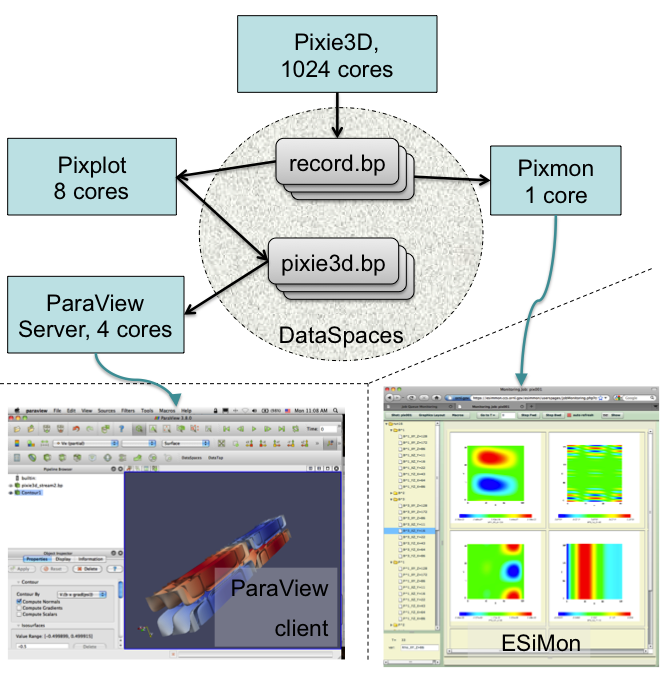
\includegraphics[width=0.5\textwidth]{Chapters/part3-ch5-adios/figs/intransitviz.png}
}
{
% use B&W version
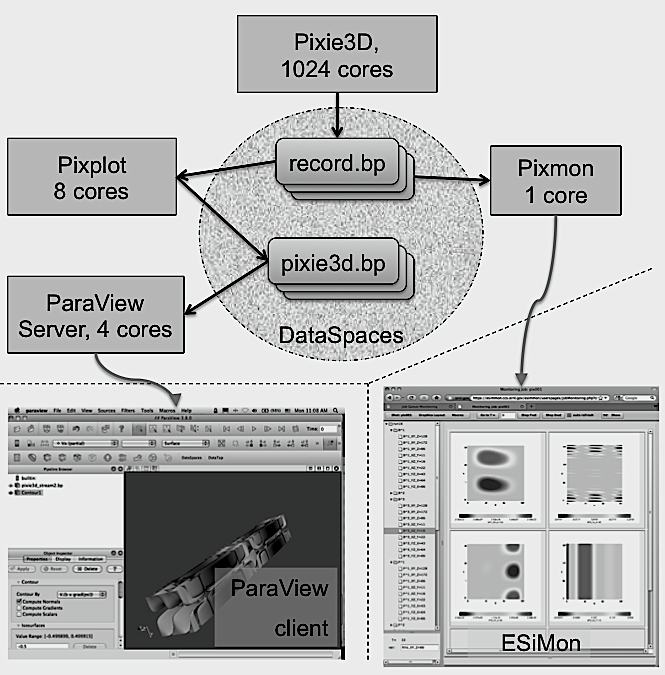
\includegraphics[width=0.5\textwidth]{Chapters/part3-ch5-adios/figs/intransitviz-bw.png}
}
\caption[]
{In~transit analysis and visualization pipeline using ADIOS.
}
\label{part3-ch5-adios:fig:intransitviz}
\end{figure}

The application codes are written as if writing data to files and reading data from files, processing one step at a time and only advancing forward in time. ADIOS allows for a seamless switch from file-based post-processing to online processing helped with memory-to-memory data transfers. Staging methods that transfer data directly from the memory of the producer into the memory of the consumer are best for coupling and for straight analytical pipelines (e.g. DIMES and FlexPath methods of ADIOS). The DataSpaces model~\cite{ADIOS:Docan:cluster12}, however, provides a virtual shared multi-dimensional space using a set of separate nodes as a ``staging area,". Thus multiple, parallel applications can simultaneously read a multi-dimensional array, with an arbitrary decomposition. More importantly for interactive visualization, DataSpaces can hold as many output steps as the allocated memory can hold and can serve a reader with data the producer long has forgotten about. Moreover, DataSpaces provides fault isolation for the application. Failures downstream in a process pipeline does not propagate to the application. More details on using ADIOS and DataSpaces for in-transit visualization can be found in the book on High Performance Visualization~\cite{ADIOS:Bethel-Childs-Hansen:HPV:2012}.



\subsection{Code coupling}
{\color {red}Manish: use Fusion as example}
%\subsubsection*{Plasma Fusion simulations}

The largest community that uses ADIOS is of the plasma fusion simulations, as several fusion scientists have been collaborating with the ADIOS team and used the library in their applications from the beginning, giving invaluable insight for the ADIOS team in the works of many large scale simulations. Particle simulation based fusion applications that can utilize the largest  supercomputers (i.e. several hundreds of thousands of cores today), like XGC1, GTC and GTC-P all use ADIOS for writing the large checkpoint/restart data as well as the small but frequent diagnostic data. ADIOS played center role in coupling multiple fusion codes together for creating a multi-scale multi-physics fusion simulation~\cite{ADIOS:Docan:ccgrid10}. The separate codes used ADIOS to write and read data that was transferred between the codes directly without writing files. Magneto-hydrodynamic codes like M3D-K, M3D-C1 and GEM also use ADIOS for checkpoint/restart because they had I/O bottlenecks already at a few hundred cores. The output of M3D was also changed to ADIOS in order to feed that data into XGC in a fusion coupling scenario. 





\subsection{Data reduction}
{\color {red}Nagiza: PARLO}
Application of data reduction techniques with ADIOS have shown to be effective in reducing the
bottleneck on I/O during simulation writes. These techniques fit well with the minimal communication
principle employed by ADIOS, where each process handles its own I/O. By applying compression
routines locally on every process, encoding costs are effectively minimized. This also enables
compression techniques to take advantage of similarity in data values within each process, typically
seen with spatio-temporal scientific datasets. For example, ISOBAR \cite{ADIOS:Schendel2012b}, an in situ
lossless compression routine specific for scientific data, demonstrated up to a 46\% reduction in
storage on datasets from simulations spanning various domains such as combustion (S3D), plasma
(XGC1, GTS) and astrophysics (FLASH). This technique coupled with ADIOS and with the addition of
interleaving allowed throughput gains proportional to the degree of data reduction.

While checkpoint/restart data such as particle data must be compressed losslessly, datasets that are
used for analysis and visualization, such as field data, can be compressed in a lossy fashion.
Unlike lossless compression, lossy compression techniques such as wavelets-based compression,
ISABELA \cite{ADIOS:Lakshminarasimhan2013a}, etc. provide a multi-fold reduction in storage sizes, trading
precision for reduced storage. Depending on the sensitivity of the analysis routines to errors
introduced by the compression process, the end-users can change the level of accuracy desired in the
configuration file used by ADIOS. The configuration file can also instruct ADIOS to employ different
compression routines for different variables and output groups (checkpoint/restart or analysis),
without having to change the application code.





\subsection{Deployment}
ADIOS is an open source software with a BSD license. It has been installed as central software and is supported organizationally by the OLCF, by the iVEC organization in Western Australia for the purpose of supporting the Square-Kilometer Array project, by the High Level Support Team (HLST) supporting EFDA (European Fusion Development Agreement) sites, and by the ERDC center of the US. Army Corps of Engineers. At other locations, application scientists install ADIOS themselves for their own application. Many of those receive guidance from the ADIOS team located at the OLCF to utilize their target system optimally.



\index{Data Formats}
\index{I/O middleware}


\section{Conclusion}
{\color {red}Scott}
{\color {red}Summary of experiences with the library. Future challenges and directions.}

%This is a reference to a book chapter~\ref{ch0:book-intro}.
%This is a reference to a bibtex item~\cite{Snir:MPI}.}

\putbib[Chapters/part3-ch5-adios/part3-ch5-adios]
